\chapter{Bibliograf\'{\i}a, Figuras, Tablas y Ecuaciones}

La Norma T\'{e}cnica Colombiana NTC 1486 fija la reglamentaci\'{o}n nacional para la ``presentaci\'{o}n de tesis, trabajos de grado y otros trabajos de investigaci\'{o}n'' \citep{NTC1486}. Se recomienda a los autores revisar cuidadosamente la Norma para familiarizarse con su contenido antes de empezar a escribir su propio documento. Pero adem\'{a}s, se recomienda mantener el documento a mano como fuente de referencia permanente. \\

Por otra parte, la Norma T\'{e}cnica Colombiana NTC 5613 se refiere a las referencia bibliogr\'{a}ficas, su contenido, forma y estructura \citep{NTC5613}. En esta plantilla se recogen las ideas generales de la Norma NTC 5613, para lo cual se utiliza el estilo de citas \emph{agsm} (tipo autor-a\~{n}o), tomado de la familia de estilos bibliogr\'{a}ficos \emph{Harvard} \citep{Harvard:2008}, pero usando el paquete de referencias y citas para las ciencias naturales \emph{Natbib} \citep{Natbib:2010, Natbib:2010RS}. \\

Las figuras, tablas y ecuaciones se enumeran consecutivamente dentro de cada cap\'{\i}tulo. \\

Las siguientes secciones de este cap\'{\i}tulo describen c\'{o}mo citar las referencias bibliogr\'{a}ficas y como referenciar en el texto las figuras, las tablas y las ecuaciones.

\section{Citas bibliogr\'{a}ficas}

En primer lugar, se debe crear un archivo con todas las referencias bibliogr\'{a}ficas. En esta plantilla este archivo tiene la extensi\'{o}n \emph{bib} y se llama \emph{BiblioPAE}. Los archivos tipo \emph{bib} tienen entradas que el programa {\textsc{Bib}}{\TeX} interpreta e incorpora en el documento final. \\

Por ejemplo, la cita del trabajo \citet{Harvard:2008} se introduce en el archivo BiblioPAE.bib de la siguiente manera:

\begin{verbatim}
	@Manual{Harvard:2008,
	title = {The {H}arvard {F}amily of {B}ibliography {S}tyles},
	author = {Peter Williams and Thorsten Schnier},
	month = {Noviembre},
	year = {2008},
	note = {ftp://ftp.tex.ac.uk/tex-archive/macros/latex/contrib/harvard/harvard.pdf},
}
\end{verbatim}

Dependiendo de la forma en que se introduzca la cita, \'{e}sta lucir\'{a} de manera diferente. Por ejemplo, si se usa
\verb"\citet{Harvard:2008}", la referencia ser\'{a}  adecuada para una expresi\'{o}n de la forma: ``... de acuerdo con \citet{Harvard:2008}...'' \\

Pero si se usa
\verb"\citep{Harvard:2008}", la referencia ser\'{a} m\'{a}s adecuada para la expresi\'{o}n: ``... si se usa el estilo \emph{Harvard} \citep{Harvard:2008}...'' \\

Para otras variaciones de la forma de citar, consulte el manual de \emph{Natbib} \citep{Natbib:2010}. \\

Los siguientes ejemplos pueden resultar \'{u}tiles para ilustrar la forma de citar en el documento:

\begin{itemize}

\item El sistema de procesamiento estad\'{\i}stico de libre distribuci\'{o}n \emph{\textbf{R}} \citep{R} se utiliza para ejecutar el procesamiento de los datos en este Trabajo de Grado.

\item En este Trabajo de Grado se utiliza la librer\'{\i}a Lattice de \emph{\textbf{R}} \citep[ver][]{Sarkar:2008}.

\item Seg\'{u}n \citet{Wood:2003}, la suavizaci\'{o}n spline es una de las t\'{e}cnicas m\'{a}s comunes para estimar la funci\'{o}n de regresi\'{o}n en los m\'{e}todos de regresi\'{o}n no param\'{e}trica.

\item El modelo de regresi\'{o}n lineal podr\'{\i}a considerarse el m\'{e}todo estad\'{\i}stico m\'{a}s utilizado en el an\'{a}lisis de datos \citep{Graybill:1976, Draper:Smith:1998, Neter:1990, Seber:1977, Searle:1971}.

\item \citet[p\'{a}g. 12]{Eubank:1999} presenta la idea b\'{a}sica del concepto de  \emph{suavizaci\'{o}n}.

\end{itemize}

\section{Presentaci\'{o}n y citaci\'{o}n de figuras}

Las ilustraciones forman parte del contenido de los cap\'{\i}tulos. Se deben colocar en la misma p\'{a}gina en que se mencionan o en la siguiente (deben siempre mencionarse en el texto).\\

Un ejemplo para la presentaci\'{o}n y citaci\'{o}n de figuras, se presenta a continuaci\'{o}n (citaci\'{o}n directa):\\

La Figura \ref{Fi} presenta un histograma del costo total bajo la politica PRW, los histogramas bajo las dos aproximaciones sugieren una mezcla de sub-poblaciones.

\begin{figure}
\centering
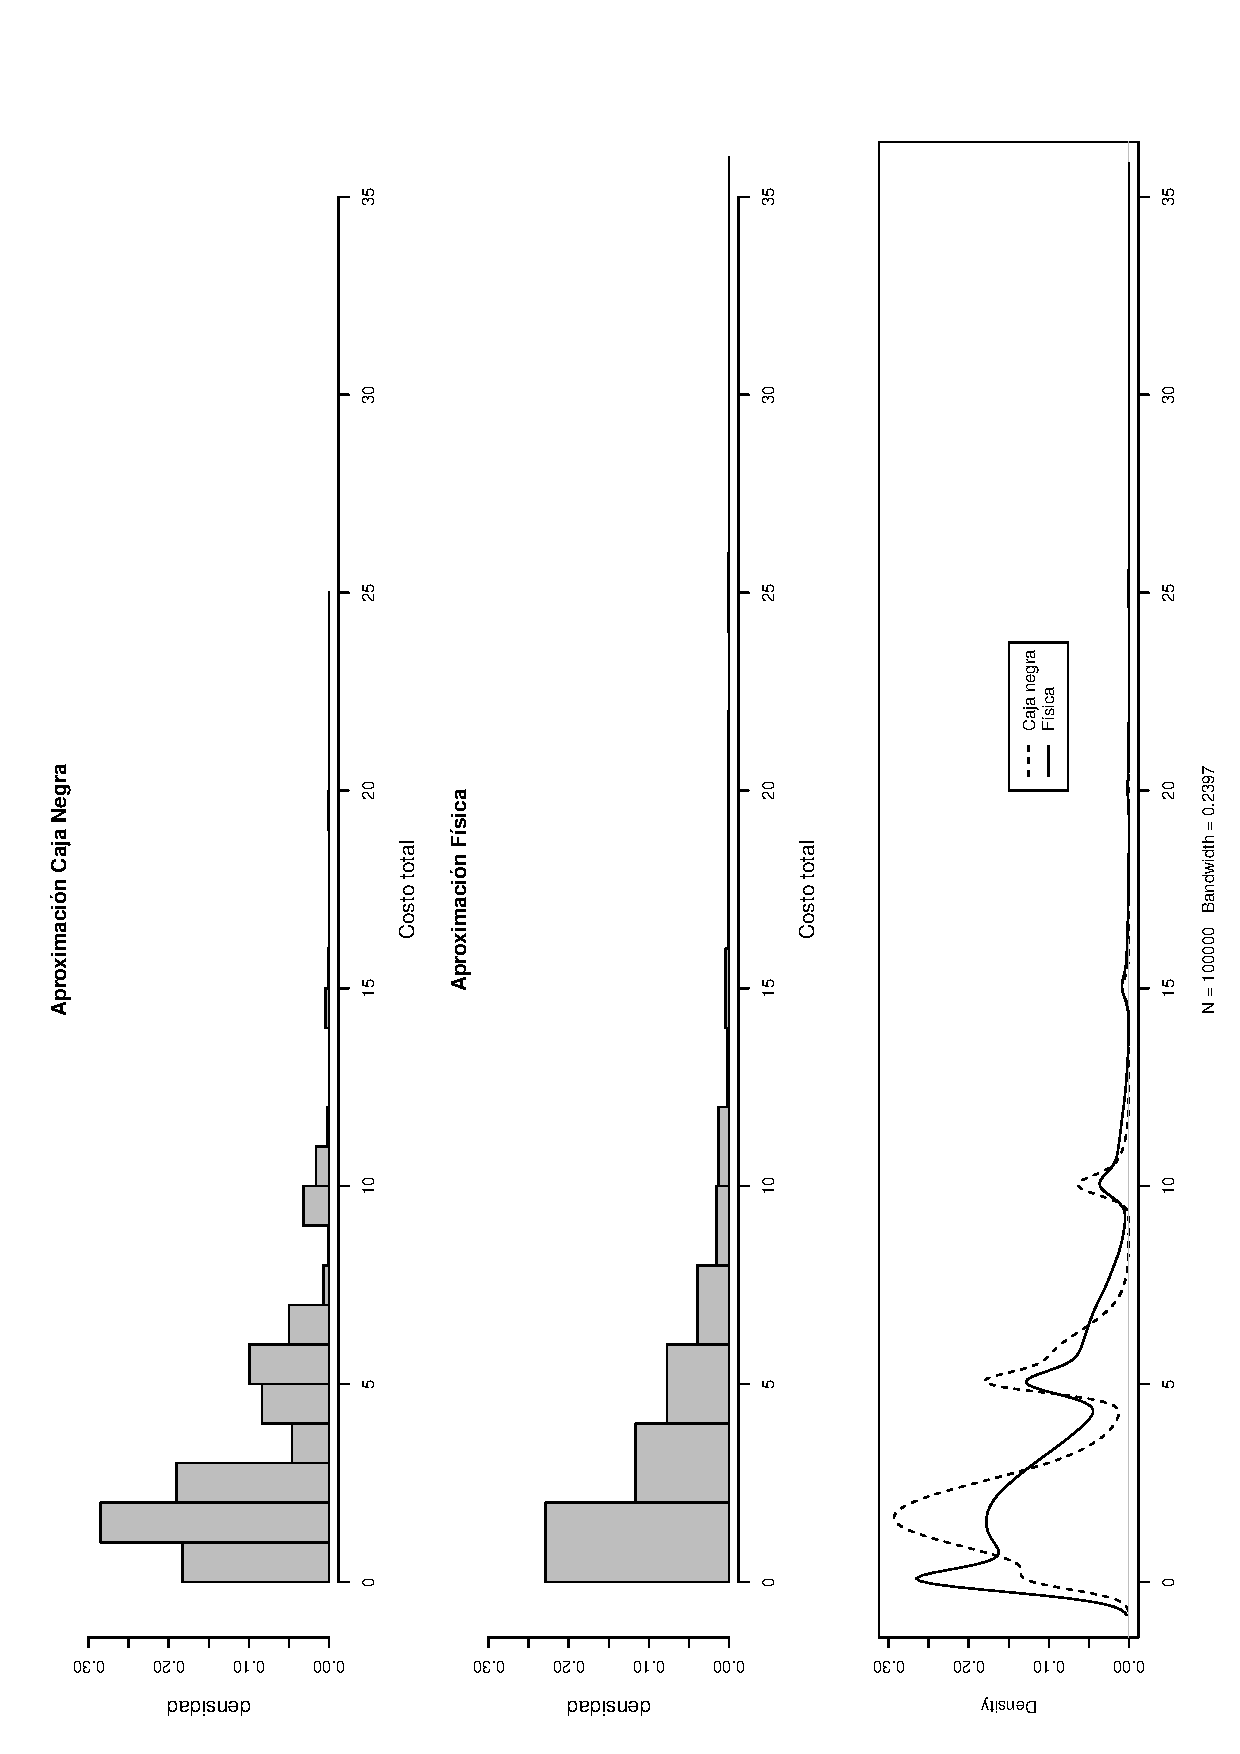
\includegraphics[scale=0.4, angle=-90]{Kap3/Fig_Cap3/Costo_Total}
\caption{Histograma de costos totales de garant\'{\i}a. Pol\'{\i}tica PRW.} \label{Fi}
\end{figure}

\subsection*{Acerca de las notas al pie}

En general se evitar\'{a} el uso de llamadas fuera del texto principal para introducir aclaraciones o complementos. Pero en la situaci\'{o}n eventual de que esto se necesite (algo altamente improbable) estas llamadas deben hacerse con un nota al pie\footnote{ Solo en caso de necesidad extrema, las notas se usar\'{\i}an como ``notas al pie". Se utilizan para explicar, comentar o hacer referencia al texto de un documento, as\'{\i} como para introducir comentarios detallados. \emph{Las notas al pie no se usan en este informe final de Trabajo de Grado para introducir referencias bibliogr\'{a}ficas}.}.\\

La fuente documental se debe escribir al final de la figura con los elementos de la referencia (de acuerdo con las normas seleccionadas) y no como pie de p\'{a}gina. \\

\section{Presentaci\'{o}n y citaci\'{o}n de tablas}

Para la edici\'{o}n de tablas, cada columna debe llevar su t\'{\i}tulo; la primera palabra se debe escribir con may\'{u}scula inicial y preferiblemente sin abreviaturas. En las tablas y cuadros, los t\'{\i}tulos y datos se deben ubicar entre l\'{\i}neas horizontales y verticales cerradas (como se realiza en esta plantilla).\\

La numeraci\'{o}n de las tablas se realiza de la misma manera que las figuras o ilustraciones, a lo largo de todo el texto. Deben llevar un t\'{\i}tulo breve, que concreta el contenido de la tabla; \'{e}ste se debe escribir en la parte superior de la misma. Para la presentaci\'{o}n de cuadros, se deben seguir las indicaciones dadas para las tablas.\\

Un ejemplo para la presentaci\'{o}n y citaci\'{o}n de tablas (citaci\'{o}n indirecta), se presenta a continuaci\'{o}n:\\
\\
Los resultados de la prueba chi-cuadrado sugieren fuerte evidencia para rechazar la hip\'{o}tesis nula de igualdad distribucional. Ver Tabla \ref{Ta} \\

\begin{table}[htbp]
\centering
\caption{Prueba Chi-cuadrado de igualdad distribucional entre aproximaci\'{o}n caja negra y aproximaci\'{o}n f\'{\i}sica. Pol\'{\i}tica FRW.} \label{Ta}
\begin{tabular}{|c|c|c|c|} \hline              
  & $\chi^{2}$  & df   & valor-p  \\\hline
costo falla I & 12379.12 & 6 & $< 2.2 \times 10^{-16}$ \\\hline
costo falla II & 5893.437 & 17 & $< 2.2 \times 10^{-16}$ \\\hline
costos total & 10700.75 & 26 & $< 2.2 \times 10^{-16}$  \\\hline
\end{tabular}%
\end{table}

\textbf{NOTA:} en el caso en que el contenido de la tabla sea muy extenso, se puede cambiar el tama\~{n}o de la letra, siempre y cuando \'{e}sta sea visible por el lector.\\

\subsection{Consideraciones adicionales para el manejo de figuras, tablas y ecuaciones}
Cuando una tabla, cuadro o figura ocupa m\'{a}s de una p\'{a}gina, se debe repetir su identificaci\'{o}n num\'{e}rica, seguida por la palabra continuaci\'{o}n.\\

Adicionalmente los encabezados de las columnas se deben repetir en todas las p\'{a}ginas despu\'{e}s de la primera.\\

Los anteriores lineamientos se contemplan en la presente plantilla.\\

\begin{itemize}
\item Presentaci\'{o}n y citaci\'{o}n de ecuaciones.
\end{itemize}

La citaci\'{o}n de ecuaciones, en caso que se presenten, debe hacerse como lo sugiere esta plantilla. Todas las ecuaciones deben estar numeradas y citadas detro del texto.\\

Para el manejo de cifras se debe seleccionar la norma seg\'{u}n el \'{a}rea de conocimiento del trabajo de grado. \\

\begin{equation}\label{procFRW_bb}
Z_{w}^{FRW}= \sum_{j=1}^{\eta} \left( c^{I} N_{T^{II}_{j}}^{I} + c^{II}\right) -\left( c^{I} N_{T^{II}_{\eta}}^{I} + c^{II} \right) + c^{I} N_{w}^{I}
\end{equation}

y el valor esperado del proceso de costo (\ref{procFRW_bb}) se encuentra dado por,

\begin{equation}\label{esperanza_FRW_bb}
E\left( Z_{w}^{FRW}\right) = E\left[ \sum_{j=1}^{\eta} \left(c^{I} N_{T^{II}_{j}}^{I} + c^{II}\right) - \left(c^{I} N_{T^{II}_{\eta}}^{I} + c^{II}\right)    \right]   + E \left[  c^{I} N_{w}^{I}\right] 
\end{equation}

Para obtener la expresi\'{o}n del valor esperado del proceso de costo $Z_{w}^{FRW}$ en (\ref{esperanza_FRW_bb}) se realiza el c\'{a}lculo de la esperanza para cada uno de los t\'{e}rminos que componen la expresi\'{o}n.